\documentclass[../main.tex]{subfiles}
\begin{document}
实数域上的内积空间上的厄米算符、反厄米算符和幺正算符分别特称为对称算符、斜称算符和正交算符。它们的定义方式与其在复数域上的对应是一样的,但它们的部分性质与其在复数域上的对应不同。最突出的表面是那些通过特征多项式和行列式得出的性质。

我们在上一节看到,$n$维欧几里得空间的平移空间是一个实数域$\mathbb{R}$上的$n$维内积空间;欧几里得空间上的几何规律已经由向量内积的性质和欧几里得范的性质得以确定。当实数域$\mathbb{R}$上的一个$n$维内积空间$\mathcal{V}$是$n$维欧几里得空间$\mathcal{E}$的平移空间时,$\mathcal{V}$上的对称算符、斜称算符和正交算符对$\mathcal{V}$中的向量作用的结果,将对应于欧几里得空间中的几何形状的变换。

本节我们讨论这三种算符在3维欧几里得空间上的特殊性质和由此得出的几何意义。

\subsection{正交算符}\label{sec:II.3.3.1}
首先,由定理\ref{thm:II.2.34},在$n$维实内积空间上的任一正交算符的行列式要么等于$1$要么等于$-1$。于是正交算符可按此分为两类,需要分开讨论。

我们先在2维的情况上认识正交算符。

\subsubsection{2维欧几里得平面上的正交算符}
设$\mathcal{V}$是2维欧几里得空间的平移空间,$\mathbf{Q}$是$\mathcal{V}$上的一个正交算符。设基本坐标系对应$\mathcal{V}$的一组基是$B^\prime=\left(\mathbf{\hat{e}}^\prime_1,\mathbf{\hat{e}}^\prime_2\right)$,则$\mathbf{Q}$在$B^\prime$下的坐标矩阵可记为
\[\left(\mathbf{Q}\right)_{B^\prime}=\left(\begin{array}{cc}Q_{11}&Q_{12}\\Q_{21}&Q_{22}\end{array}\right)\]
由线性算符在给定基下的坐标计算式、正交算符在内积运算中的性质、以及正交算符行列式的性质可得
\begin{align*}
    \mathbf{QQ}^\intercal=\mathbf{I} & \Leftrightarrow
    \left\{\begin{aligned}Q_{11}^2+Q_{12}^2=Q_{21}^2+Q_{22}^2 & =1 \\
               Q_{11}Q_{21}+Q_{12}Q_{22}           & =0\end{aligned}\right.                  \\
    \mathrm{det}\mathbf{Q}=\pm 1     & \Leftrightarrow Q_{11}Q_{22}-Q_{12}Q_{21}  =\pm 1
\end{align*}
其中“$\pm$”表示当$\mathrm{det}\mathbf{Q}=1$时取正号,当$\mathrm{det}\mathbf{Q}=-1$时取负号。由上列关系可推出,存在一个角度$\theta\in\left[0,2\pi\right]$,使得
\[Q_{11}=\cos\theta,\quad Q_{12}=\sin\theta,\quad Q_{21}=\cos\phi,\quad Q_{22}=\sin\phi\]
且有
\begin{align*}
    Q_{11}Q_{21}+Q_{12}+Q_{22}  =0    & \Leftrightarrow\cos\left(\phi-\theta\right)=0     \\
    Q_{11}Q_{22}-Q_{12}Q_{21}  =\pm 1 & \Leftrightarrow\sin\left(\phi-\theta\right)=\pm 1
\end{align*}
由这两个等式可以得到$\phi=\theta\pm\pi/2$。因此,$\mathbf{Q}$总可由某角$\theta$表示成以下形式
\[\left(\mathbf{Q}\right)_{B^\prime}=\left(\begin{array}{cc}\cos\theta&\sin\theta\\\mp\sin\theta&\pm\cos\theta\end{array}\right)\]

下面我们考察$\mathbf{Q}$作用于任一给定向量$\mathbf{a}\in\mathcal{V}$的几何效果。$\mathbf{a}$在基$B^\prime$下的坐标表达式是$\mathbf{a}=\alpha_1\mathbf{\hat{e}}^\prime_1+\alpha_2\mathbf{\hat{e}}^\prime_2$。

当$\mathrm{det}\mathbf{Q}=1$时,$\mathbf{Qa}$的坐标由下式计算得到
\[\left(\mathbf{Qa}\right)_{B^\prime}=\left(\begin{array}{cc}\cos\theta&\sin\theta\\-\sin\theta&\cos\theta\end{array}\right)\left(\begin{array}{c}\alpha_1\\\alpha_2\end{array}\right)=\left(\begin{array}{c}\alpha_1\cos\theta+\alpha_2\sin\theta\\-\alpha_1\sin\theta+\alpha_2\cos\theta\end{array}\right)\]
由正交算符的性质,$\left\|\mathbf{Qa}\right\|=\left\|\mathbf{a}\right\|$,故我们仅需关心$\mathbf{Qa}$与$\mathbf{a}$的夹角$\omega$,由角的定义,利用矩阵运算,可得
\[
    \cos\omega=\frac{\left(\mathbf{Qa}|\mathbf{a}\right)}{\left(\mathbf{a}|\mathbf{a}\right)}=\cos\theta
\]
由定义\ref{def:II.3.6},夹角$\omega$的取值范围是$\left[0,\pi\right]$,而$\theta\in\left[0,2\pi\right]$。实际上$\mathbf{Qa}$相对于$\mathbf{a}$可旋转的角度根据$\theta$的取值范围,可以完整地转一圈。$\theta$是由所讨论的正交算符$\mathbf{Q}$确定的。给定一个特定的正交算符,就对应着特定角度$\theta$值的旋转操作。值得注意的是,随着$\theta$的增加,$\mathbf{Qa}$相对$\mathbf{a}$的旋转方向是由$\mathbf{\hat{e}}^\prime_2$到$\mathbf{\hat{e}}^\prime_1$,在通常的作图惯例中是“顺时针”旋转的。

总之,当$\mathrm{det}\mathbf{Q}=1$时,任一向量$\mathbf{a}$在被$\mathbf{Q}$作用之后,长度不变,方向变化角度$\theta$(如图\ref{fig:II.3.1}),$\theta$的取值由$\mathbf{Q}$确定。

\begin{figure}[ht]
    \centering
    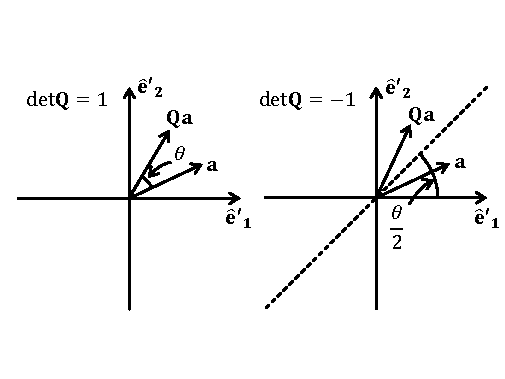
\includegraphics[width=0.5\textwidth]{images/II.3.1.pdf}
    \caption{正交算符在2维欧几里得平面中的几何意义。}
    \label{fig:II.3.1}
\end{figure}

接下来我们考虑$\mathrm{det}\mathbf{Q}=-1$时的情况。由定理\ref{thm:II.2.35}$\mathcal{V}$中必有一组基$B=\left(\mathbf{\hat{e}}_1,\mathbf{\hat{e}}_2\right)$使$\mathbf{Q}$的坐标矩阵是对角矩阵$\mathrm{diag}\left(\lambda_1,\lambda_2\right)$。又由$\mathbf{Q}$的行列式性质,在实数域上$\lambda_i=\pm 1,i=1,2$,因此可以确定$\lambda_1=1$、$\lambda_2=-1$,$\mathbf{Q}$在$B$下的坐标矩阵就是
\[\left(\mathbf{Q}\right)_B=\left(\begin{array}{cc}1&0\\0&-1\end{array}\right)\]
这组基$B$是由$\mathbf{Q}$的性质规定的,一般不会恰巧就与基本坐标系的基$B^\prime$重合。设$P$是由$\mathbf{B}$到$\mathbf{B}^\prime$的过渡矩阵,则$P$也应是一个正交矩阵。按照之前的结论,矩阵$P$可以某角度$\phi$表示成
\[P=\left(\begin{array}{cc}\cos\phi&\sin\phi\\\mp\sin\phi&\pm\cos\phi\end{array}\right)\]

事实上$\phi$是$\mathbf{\hat{e}}^\prime_1$与$\mathbf{\hat{e}}_1$的夹角。诚然,
\begin{align*}
    \left(\mathbf{\hat{e}}^\prime_1|\mathbf{\hat{e}}_1\right) & =\left(\sum_{k=1}^2P_{k1}\mathbf{\hat{e}}_k|\mathbf{\hat{e}}_1\right) \\
                                                              & =\sum_{k=1}^2P_{1k}\left(\mathbf{\hat{e}}_k|\mathbf{\hat{e}}_1\right) \\
                                                              & =\sum_{k=1}^2P_{1k}\delta_{k1}=P_{11}=\cos\phi
\end{align*}

由之前的结论,$\mathbf{Q}$在$B^\prime$下的坐标可用某角$\theta$表示,同时又是通过矩阵$P$从其在$B$下的坐标变换而来的,故有以下关系
\begin{align*}
    \left(\mathbf{Q}\right)_{B^\prime} & =\left(\begin{array}{cc}\cos\theta&\sin\theta\\\sin\theta&-\cos\theta\end{array}\right) \\
                                       & =P^{\intercal}\left(\mathbf{Q}\right)_BP                                                \\
    \Leftrightarrow                    & \phi=\theta/2
\end{align*}

现在,$\mathbf{Qa}$在$B^\prime$下的坐标可由坐标运算得到

\[
    \begin{aligned}
        \left(\mathbf{Qa}\right)_{B^\prime} & =\left(\begin{array}{c}\alpha_1\cos\theta+\alpha_2\sin\theta\\-\alpha_2\cos\theta+\alpha_1\sin\theta\end{array}\right)           \\
                                            & =\left\|\mathbf{a}\right\|\left(\begin{array}{c}\cos\left(\theta-\delta\right)\\\sin\left(\theta-\delta\right)\end{array}\right)
    \end{aligned}
\]
其中$\tan\delta=\alpha_2/\alpha_1$,即$\delta$是$\mathbf{a}$与$\mathbf{\hat{e}}^\prime_1$的夹角,上式又说明$\mathbf{Qa}$与$\mathbf{\hat{e}}^\prime_1$的夹角是$\theta-\delta$。通过角度关系可以发现,$\mathbf{Qa}$与$\mathbf{a}$关于角度为$\theta/2$的对称轴镜象翻转,其中“角度”是指与所选定规范正交基的第1个单位基向量的夹角(图\ref{fig:II.3.1})。$\theta$是$\mathbf{Q}$在所选定的规范正交基下的坐标矩阵取前文所述的表达式时的角;它是$\mathbf{Q}$本身的特性。也就是说,当$\mathrm{det}\mathbf{Q}=-1$时,$\mathbf{Q}$在2维欧几里得空间中确定了一条对称轴,并将原向量$\mathbf{a}$关于该对称轴镜象翻转。随着$\theta$在其取值范围$\left[0,2\pi\right]$变化,$\mathbf{Qa}$相对于原向量$\mathbf{a}$关于一条旋转的对称轴镜象翻转,而实际表现为一定角度的表观旋转。

\subsubsection{3维欧几里得空间上的正交算符}
设$\mathbf{Q}$是3维欧几里得空间$\mathcal{E}$的平移空间$\mathcal{V}$上的正交算符。由正交算符的行列式的性质可知其3个特征值$\lambda_i=\pm 1,i=1,2,3$。在$\mathcal{V}$中可以选出关于$\mathbf{Q}$的第1个特征值$\lambda_1$的单位特征向量$\mathbf{\hat{e}}_1$,并且总可以在$\mathcal{V}$中再找出两个单位向量$\mathbf{\hat{e}}_2$、$\mathbf{\hat{e}}_3$与$\mathbf{\hat{e}}_1$形成一组规范正交基$B=\left(\mathbf{\hat{e}}_1,\mathbf{\hat{e}}_2,\mathbf{\hat{e}}_3\right)$。

一般地,一个算符$\mathbf{Q}$在一个规范正交基下的坐标$Q_{ij}$,是可以通过与相应的单位基向量形成内积而得到的:$Q_{ij}=\left(\mathbf{Q}\mathbf{\hat{e}}_i|\mathbf{\hat{e}}_j\right)$(这是容易验证的)。所以我们可以得出以下几个等式:
\[\begin{aligned}
        Q_{11} & =\left(\mathbf{Q}\mathbf{\hat{e}}_1|\mathbf{\hat{e}}_1\right)=\lambda_1=\pm 1                                                                                                        \\
        Q_{12} & =\left(\mathbf{Q}\mathbf{\hat{e}}_1|\mathbf{\hat{e}}_2\right)=Q_{13}=\left(\mathbf{Q}\mathbf{\hat{e}}_1|\mathbf{\hat{{e}}}_3\right)=0                                                \\
        Q_{21} & =\left(\mathbf{Q}\mathbf{\hat{e}}_2|\mathbf{\hat{e}}_1\right)=\left(\mathbf{\hat{e}}_2|\mathbf{Q}^*\mathbf{\hat{e}}_1\right)=\pm\left(\mathbf{\hat{e}}_2|\mathbf{\hat{e}}_1\right)=0
    \end{aligned}\]
其中,第三个等式利用到事实$\mathbf{Q}^*\mathbf{\hat{e}}_1=\pm\mathbf{\hat{e}}_1$,因为
\[\mathbf{\hat{e}}_1=\mathbf{Q}^*\mathbf{Q}\mathbf{\hat{e}}_1=\mathbf{Q}^*\left(\pm\mathbf{\hat{e}}_1\right)=\pm\mathbf{Q}^*\mathbf{\hat{e}}_1\]
同理有
\[\left(\mathbf{Q\hat{e}}_3|\mathbf{\hat{e}}_1\right)=0\]
另外注意到,$\left(\mathbf{Q\hat{e}}_i|\mathbf{\hat{e}}_j\right)$同时也是向量$\mathbf{Q\hat{c}}_i$的第$j$个坐标,故可知
\[\mathbf{Q\hat{e}}_2=Q_{22}\mathbf{\hat{e}}_2+Q_{23}\mathbf{\hat{e}}_3,\quad\mathbf{Q\hat{e}}_3=Q_{32}\mathbf{\hat{e}}_2+Q_{33}\mathbf{\hat{e}}_3\]
再由$\left\|\mathbf{Q\hat{e}}_2\right\|=\left\|\mathbf{\hat{e}}_2\right\|=\left\|\mathbf{Q\hat{e}}_3\right\|=\left\|\mathbf{\hat{e}}_3\right\|=1$有
\[Q_{22}^2+Q_{23}^2=Q_{32}^2+Q_{33}^2=1\]
再由$\left(\mathbf{\hat{e}}_2|\mathbf{\hat{e}}_3\right)=0$有
\[Q_{22}Q_{32}+Q_{23}Q_{33}=0\]
再由$\mathrm{det}\mathbf{Q}=\pm 1$有
\[-Q_{23}Q_{32}+Q_{22}Q_{33}=\pm 1\]
总结上述讨论,我们通过正交算符的一般性质,得到了$\mathbf{Q}$的分量的最具体结论如下
\[
    \begin{array}{l}
        Q_{11}                     =\pm 1,             \\
        Q_{12}=Q_{13}=Q_{21}=Q_{31}=0                  \\
        Q_{22}^2+Q_{23}^2         =Q_{32}^2+Q_{33}^2=1 \\
        Q_{22}Q_{32}+Q_{23}Q_{33} =0
    \end{array}
\]
其中最后两个等式跟2维的情况是很类似的,可用某角$\theta\in\left[0,2\pi\right]$表达成
\[\left(\mathbf{Q}\right)_B=\left(\begin{array}{ccc}\pm 1&0&0\\0&\cos\theta&\sin\theta\\0&\mp\sin\theta&\pm\cos\theta\end{array}\right)\]
其中“$\pm$”表示当$\mathrm{det}\mathbf{Q}=1$时取正号,当$\mathrm{det}\mathbf{Q}=-1$时取负号。

以下我们考察,对任意向量$\mathbf{a}\in\mathcal{V}$,$\mathbf{Qa}$相比于$\mathbf{a}$在以$\mathcal{V}$为平移空间的欧几里得空间中的效果。我们记$\mathbf{a}$在基$B$下的坐标是$\left(\alpha_1,\alpha_2,\alpha_3\right)$。

当$\mathrm{det}\mathbf{Q}=1$时,易验$\left(\mathbf{Qa}|\mathbf{\hat{e}}_1\right)=\left(\mathbf{a}|\mathbf{\hat{e}}_1\right)$,也就是说,$\mathbf{Q}$的作用不改变向量与$\mathbf{\hat{e}}_1$的夹角。具体地,$\mathbf{Qa}$的坐标表达式是
\[\left(\mathbf{Qa}\right)_B=\left(\begin{array}{c}\alpha_1\\\alpha_2\cos\theta+\alpha_3\sin\theta\\-\alpha_2\sin\theta+\alpha_3\cos\theta\end{array}\right)\]
比较行列式为1的正交算符在2维欧几里得平面的结果,上式的后两项表示向量$\alpha_2\mathbf{\hat{e}}_2+\alpha_3\mathbf{\hat{e}}_3$在$\left(\mathbf{\hat{e}}_2,\mathbf{\hat{e}}_3\right)$所确定的平面上绕原点旋转了角$\theta$。联系格拉姆--施密特正交化过程可知,$\alpha_2\mathbf{\hat{e}}_2+\alpha_3\mathbf{\hat{e}}_3$就是向量$\mathbf{a}$在$\left(\mathbf{\hat{e}}_2,\mathbf{\hat{e}}_3\right)$所确定的平面上的投影向量。

因此,行列式为1的正交算符$\mathbf{Q}$在3维欧几里得空间的效果可以总结为:$\mathbf{Q}$在3维欧几里得空间确定了一个规范正交基$B=\left\{\mathbf{\hat{e}}_1,\mathbf{\hat{e}}_2,\mathbf{\hat{e}}_3\right\}$,其中$\mathbf{\hat{e}}_1$是一个旋转轴。对任意平移向量$\mathbf{a}$,$\mathbf{Qa}$在$\mathbf{\hat{e}}_2,\mathbf{\hat{e}}_3$所张的平面上的投影相比于$\mathbf{a}$在这一平面上的投影绕旋转轴旋转角$\theta$(图\ref{fig:II.3.2})。值得注意的是,这个规范正交基$B$是由$\mathbf{Q}$的性质确定的,它未必与我们已经选定的直角坐标系$B^\prime$相重合。所以一般地,由$\mathbf{Q}$所定义的旋转轴在预先选定的直角坐标系中是“斜放”的。

\begin{figure}[ht]
    \centering
    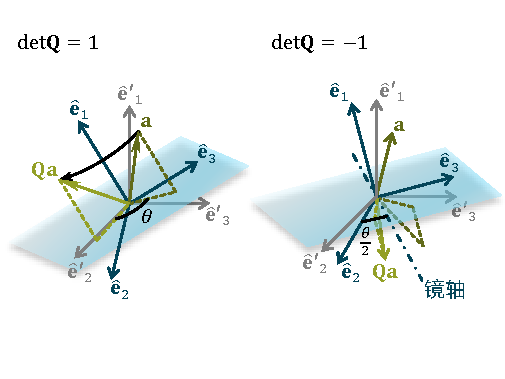
\includegraphics[width=0.5\textwidth]{images/II.3.2.pdf}
    \caption{正交算符在3维欧几里得空间中的几何意义。$B^\prime=\left(\mathbf{\hat{e}}^\prime_1,\mathbf{\hat{e}}^\prime_2,\mathbf{\hat{e}}^\prime_3\right)$是我们已经选定的直角坐标系(土黄色),$B=\left(\mathbf{\hat{e}}_1,\mathbf{\hat{e}}_2,\mathbf{\hat{e}}_3\right)$是由正交算符$\mathbf{Q}$确定的一组规范正交基(深蓝色)。在3维欧几里得空间中,$\mathbf{Q}$确定的基$B$总是由一个轴$\mathbf{\hat{e}}_1$和一个与之正交的平面$\left(\mathbf{\hat{e}}_2,\mathbf{\hat{e}}_3\right)$组成,$\mathbf{Q}$对任意向量$\mathbf{a}$的操作,都以这个轴和这个平面为基准。}
    \label{fig:II.3.2}
\end{figure}

当$\mathrm{det}\mathbf{Q}=-1$时,由类似的讨论可得
\[\left(\mathbf{Qa}\right)_B=\left(\begin{array}{c}-\alpha_1\\\alpha_2\cos\theta+\alpha_3\sin\theta\\-\alpha_3\cos\theta+\alpha_2\sin\theta\end{array}\right)\]
首先,上式的第一个分量说明,$\mathbf{Qa}$与$\mathbf{\hat{e}}_1$的夹角$\phi^\prime$跟原向量$\mathbf{a}$与$\mathbf{\hat{e}}_1$的夹角$\phi$保持$\phi^\prime=\pi-\phi$的关系,也就是说$\mathbf{Qa}$把$\mathbf{a}$关于由$\left(\mathbf{\hat{e}}_2,\mathbf{\hat{e}}_3\right)$确定的平面进行了镜象翻转。然后,比较上式后两项与2维内积空间上行列式为$-1$的正交算符的结果可知,它们是$\mathbf{a}$在由$\left(\mathbf{\hat{e}}_2,\mathbf{\hat{e}}_3\right)$所确定的平面上,以与$\mathbf{\hat{e}}_2$夹角为$\theta/2$的直线为对称轴进行平面内的镜向翻转的结果(图\ref{fig:II.3.2})。

因此,行列式为$-1$的正交算符$\mathbf{Q}$在3维欧几里得空间的效果可以总结为:$\mathbf{Q}$在3维欧几里得空间中确定了一个镜像翻转的对称面,以及在该面内的一条镜像翻转的对称轴。对任意向量$\mathbf{a}$,$\mathbf{Qa}$先相对这个对称面镜向翻转,然后其在该面上的投影以这个对称轴镜象翻转。随着$\theta$的值在$\left[0,2\pi\right]$之间变化,$\mathbf{Qa}$相对于原向量$\mathbf{a}$在镜像面的另一面,以一种镜像翻转的方向旋转。这种几何操作又叫“旋转反射”(rotoreflection)或“瑕旋转”(improper rotation)。

\subsection{对称算符与向量的拉伸}\label{sec:II.3.3.2}
由定理\ref{thm:II.2.32},复数域上的厄米算符特征值全为实数。也就是说,厄米算符的特征多项式全为实根。因此,定理\ref{thm:II.2.32}中关于复数域上厄米算符的性质,也适用于在实数域上的对称算符,包括:特征值全都是实数\cite[\S 5.3 定理3.4]{周胜林2012线性代数};对应于不同特征值的特征向量必正交\cite[\S 5.3 定理3.5]{周胜林2012线性代数};必可正交对角化\cite[\S 5.3 定理3.6]{周胜林2012线性代数};存在一组规范正交基是其特征向量。

我们从其中一个结论出发:一个对称算符的3个特征向量两两正交。设$\mathbf{U}$是3维欧几里得空间中的一个对称算符。$\mathbf{U}$的3个特征值为$\lambda_1,\lambda_2,\lambda_3$,分别对应于他们的三个单位特征向量为$\mathbf{\hat{c}}_1,\mathbf{\hat{c}}_2,\mathbf{\hat{c}}_3$,形成一个规范正交基$C=\left\{\mathbf{\hat{c}}_i\right\}$。自然地,$\left(\mathbf{U}\right)_C$是一个对角矩阵
\[
    \left(\mathbf{U}\right)_C=\left(\begin{array}{ccc}\lambda_1&0&0\\0&\lambda_2&0\\0&0&\lambda_3\end{array}\right)
\]
在实际问题中我们未必方便选择$\mathbf{U}$的特征向量作为基。在我们已选择的直角坐标系$B^\prime=\left\{\mathbf{\hat{e}}^\prime_1,\mathbf{\hat{e}}^\prime_2,\mathbf{\hat{e}}^\prime_3\right\}$下,$\left(\mathbf{U}\right)_{B^\prime}$是一个普通的对称矩阵。

给定任一向量$\mathbf{a}$,若它在基$C$下的坐标表示为$\mathbf{a}=\sum_{i=1}^3\alpha_i\mathbf{\hat{c}}_i$,则有$\mathbf{Ua}=\sum_{i=1}^3\lambda_i\alpha_i\mathbf{\hat{c}}_i$。也就是说,与原向量$\mathbf{a}$相比,$\mathbf{Ua}$是分别在各$\mathbf{\hat{c}}_i$方向进行了比例为$\lambda_i$的拉伸或压缩,其中$i=1,2,3$。因此,一个对称算符$\mathbf{U}$在3维欧几里得空间中确定了1套(3个)两两正交的拉伸方向,以及在相应方向的拉伸比。我们把对称算符$\mathbf{U}$的这组单位特征向量$\left\{\mathbf{c}_i\right\}$在欧几里得空间$\mathcal{E}$中所表示的方向称为该对称算符$\mathbf{U}$的\emph{主方向(principal direction)}。一组向量\footnote{在$\mathcal{E}$中,任何几何形状都是点的集合,而点又与位置向量一一对应,故任何几何形状都是一个向量组。}在对称算符的作用下的几何效果是在各主方向上的相应倍数的拉伸形变。具体地,在$\mathbf{c}_i$方向的拉伸比就是$\lambda_i$。在预先选定的直角坐标系$B^\prime=\left(\mathbf{\hat{e}}^\prime_1,\mathbf{\hat{e}}^\prime_2,\mathbf{\hat{e}}^\prime_3\right)$中,对称算符的主方向可能是“斜放”的。

\subsection{斜称算符与向量的“叉乘”}\label{sec:II.3.3.3}
由定理\ref{thm:II.2.32}第5条,在复数域上,反厄米算符的特征值是纯虚数或零。那么,若是在实数域上(称为斜称算符),当内积空间的维数$n$是奇数时,设$\mathbf{W}$是一个斜称算符,则有以下结果
\begin{align*}
                    & \mathrm{det}\mathbf{W}^\intercal=\mathrm{det}\mathbf{W}=\mathrm{det}\left(-\mathbf{W}\right)=\left(-1\right)^n\mathrm{det}\mathbf{W}=-\mathrm{det}\mathbf{W} \\
    \Leftrightarrow & \mathrm{det}\mathbf{W}=\prod_{i=1}^k\lambda_i=0
\end{align*}
其中我们用到了行列式的一般性质(定理\ref{thm:II.2.24})和斜称(反厄米)算符的定义\ref{def:II.2.22}。所以我们可以得到一个推论:\emph{在实数域上,当$n$为奇数时,斜称算符必有一特征值为零}。而且,上列结果也说明,当$n$为奇数时,斜称算符一定不可逆。

现具体考虑3维欧几里得空间$\mathcal{E}$的情况,改设$\mathbf{W}$是$\mathcal{E}$的平移空间$\mathcal{V}$上的一个斜称算符,则对任意$\mathbf{a}\in\mathcal{V}$,
\[\begin{aligned}\left(\mathbf{Wa}|\mathbf{a}\right)                & =\left(\mathbf{a}|\mathbf{W}^*\mathbf{a}\right)=\left(\mathbf{a}|-\mathbf{Wa}\right)=-\left(\mathbf{a}|\mathbf{Wa}\right) \\
                                                                  & =-\left(\mathbf{W}^*\mathbf{a}|\mathbf{a}\right)=-\left(-\mathbf{Wa}|\mathbf{a}\right)                                    \\
               \Leftrightarrow\left(\mathbf{Wa}|\mathbf{a}\right) & =0
    \end{aligned}\]
故被$\mathbf{W}$作用过的向量,都被投影到了与原向量垂直的平面上。至于投影了之后,有没有伸缩或旋转,要看$\mathbf{W}$的具体取值。这十分类似于以往所学过的一个向量被另一个向量“叉乘”的效果\footnote{3维实内积空间上的“叉乘”在以前的线性代数课本中又称作“向量的外积”\cite[\S3.2]{周胜林2012线性代数}。请复习其计算方法。}。事实上,我们可以从斜称算符定义“叉乘”\footnote{在本讲义中,将保持使用“叉乘”这种不正式的表述。因为正式起来,3维实内积空间上的“叉乘”是抽象代数中的不同东西在3维实内积空间上的巧合。在连续介质力学的数学语言中出现的“叉乘”,有时真的就是本节所述的几何意义,有时则是外代数/外积/楔积(如向量场的旋度)。本讲义暂时不介绍基于外代数和微分型知识,故“叉乘”运算就都由本节引入了。}。我们可通过如下定理联系二者:

\begin{theorem}\label{thm:II.3.1}
    设$\mathcal{V}$是实数域$\mathbb{R}$上的3维内积空间,$\mathbf{W}$是$\mathcal{V}$上的一个斜称算符,$\mathbf{\hat{e}}_1$是$\mathbf{W}$的关于特征值$\lambda=0$的一个特征单位向量。$\left\{\mathbf{\hat{e}}_i\right\}$是由$\mathbf{\hat{e}}_1$生成的规范正交基。对任意$\mathbf{a}\in\mathcal{V}$,可定义“叉乘”运算
    \[\mathbf{Wa}=\omega\mathbf{\hat{e}}_1\times\mathbf{a}\]
    其中$\omega=\left(\mathbf{W\hat{e}}_2|\mathbf{\hat{e}}_3\right)$。
\end{theorem}
\begin{proof}
    若记向量$\mathbf{W\hat{e}}_2=\sum_{i=1}^3\beta_i\mathbf{\hat{e}}_i$,即$\beta_i=\left(\mathbf{W\hat{e}}_2|\mathbf{\hat{e}}_i\right),\quad i=1,2,3$,则有
    \begin{align*}
        \beta_1 & =\left(\mathbf{W\hat{e}}_2|\mathbf{\hat{e}}_1\right)=-\left(\mathbf{\hat{e}}_2|\mathbf{W\hat{e}}_1\right)=\left(\mathbf{\hat{e}}_2|\mathbf{0}\right)=0     \\
        \beta_2 & =\left(\mathbf{W\hat{e}}_2|\mathbf{\hat{e}}_2\right)=-\left(\mathbf{e}_2|\mathbf{W\hat{e}}_2\right)\Leftrightarrow\beta_2=-\beta_2\Leftrightarrow\beta_2=0 \\
        \beta_3 & =\left(\mathbf{W\hat{e}}_2|\mathbf{\hat{e}}_3\right)=\omega
    \end{align*}
    因此向量$\mathbf{W\hat{e}}_2=\omega\mathbf{\hat{e}}_3$。类似的方法可得到$\mathbf{W\hat{e}}_3=-\omega\mathbf{\hat{e}}_2$。故对任意$\mathbf{a}\in\mathcal{V}$,
    \[
        \mathbf{Wa}=\alpha_1\mathbf{W\hat{e}}_1+\alpha_2\mathbf{W\hat{e}}_2+\alpha\mathbf{W\hat{e}}_3=\alpha_2\omega\mathbf{\hat{e}}_3-\alpha_3\omega\mathbf{\hat{e}}_2
    \]
    这恰为$\omega\mathbf{\hat{e}}_1\times\mathbf{a}$的结果
\end{proof}
要使用这个定理,就需要先已知$\mathbf{W}$,并找到$\mathbf{W}$在关于其零特征值的一个单位特征向量。如果我们先给定两个向量的“叉乘”$\mathbf{a}\times\mathbf{b}$,那么什么样的斜称算符$\mathbf{W}$满足$\mathbf{Wb}=\mathbf{a}\times\mathbf{b}$呢?答案作为\ref{thm:II.3.1}的推论如下。

\begin{corollary}
    设$\left\{\mathbf{\hat{e}}_i\right\}$是3维欧几里得空间$\mathcal{E}$的基本坐标系下已给定的一组有序规范正交基。给定向量$\mathbf{a}\in\mathcal{V},\mathbf{a}=\sum_{i=1}^3\alpha_i\mathbf{\hat{e}}_i$,则坐标矩阵为
    \[\left(\mathbf{W}\right)=\left(\begin{array}{ccc}0&-\alpha_3&\alpha_2\\\alpha_3&0&-\alpha_1\\-\alpha_2&\alpha_1&0\end{array}\right)\]
    的斜称算符$\mathbf{W}$满足$\mathbf{Wb}=\mathbf{a}\times\mathbf{b},\forall\mathbf{b}\in\mathcal{V}$。
\end{corollary}
该推论可利用坐标变换公式证明,留作练习。“叉乘”的性质$\mathbf{a}\times\mathbf{b}=-\mathbf{b}\times\mathbf{a}$也可通过在给定规范正交基下的坐标矩阵运算得到验证(仅限3维)。

$\mathbf{Wb}$所对应的叉乘运算$\mathbf{a}\times\mathbf{b}$的第一个向量$\mathbf{a}$是由算符$\mathbf{W}$本身确定的,称为$\mathbf{W}$的\emph{轴向量(axial vetor)}。“叉乘”的结果得到的向量,在坐标变换中的有特殊的性质。对任意$\mathbf{b}\in\mathcal{V}$,其在基本坐标系下的坐标是$\left(\beta_1,\beta_2,\beta_3\right)$。当我们反转各坐标轴的方向,即在$\left\{-\mathbf{\hat{e}}_i\right\}$下,$\mathbf{b}$的坐标将变号,变成$\left(-\beta_1,-\beta_2,-\beta_3\right)$,但是易验向量$\mathbf{a}\times\mathbf{b}$在坐标轴反转前后坐标不变号(请读者用坐标变换公式验证这两个结论)。同样的性质也导致“混合积”$\left(\mathbf{a}\times\mathbf{b}\right)\cdot\mathbf{c}$这一“标量”在坐标轴反转前后变号,而“真正的”标量的值不依赖坐标变换(定理\ref{thm:II.2.23})。这是由于向量$\mathbf{a}\times\mathbf{b}$不是一个任意给定的孤立的向量;它是向量$\mathbf{b}$在以$\mathbf{a}$为轴向量的斜称算符$\mathbf{W}$的操作下的结果。由“叉乘”所得到的向量的特殊的坐标变换性质,实际上是这个投影操作带来的。有的资料称这种“叉乘得到的向量”为\emph{赝向量(pseudo-vector)}(但这不是该概念的正式定义)。
\end{document}